\section{Results}

\subsection{Data Integrity and Perturbation Structure}

The integrity checks confirm the expected 9,201 cells and 40,295 genes
(E-MTAB-9861; \citep{jeffery2022cenpa}).
The design is moderately balanced across six perturbation conditions, with
4,356 p53-WT cells and 4,845 p53-DN cells.
CENP-A status comprises 2,915 control, 2,797 acute overexpression, and 3,489
chronic overexpression cells.

\begin{figure}[ht]
  \centering
  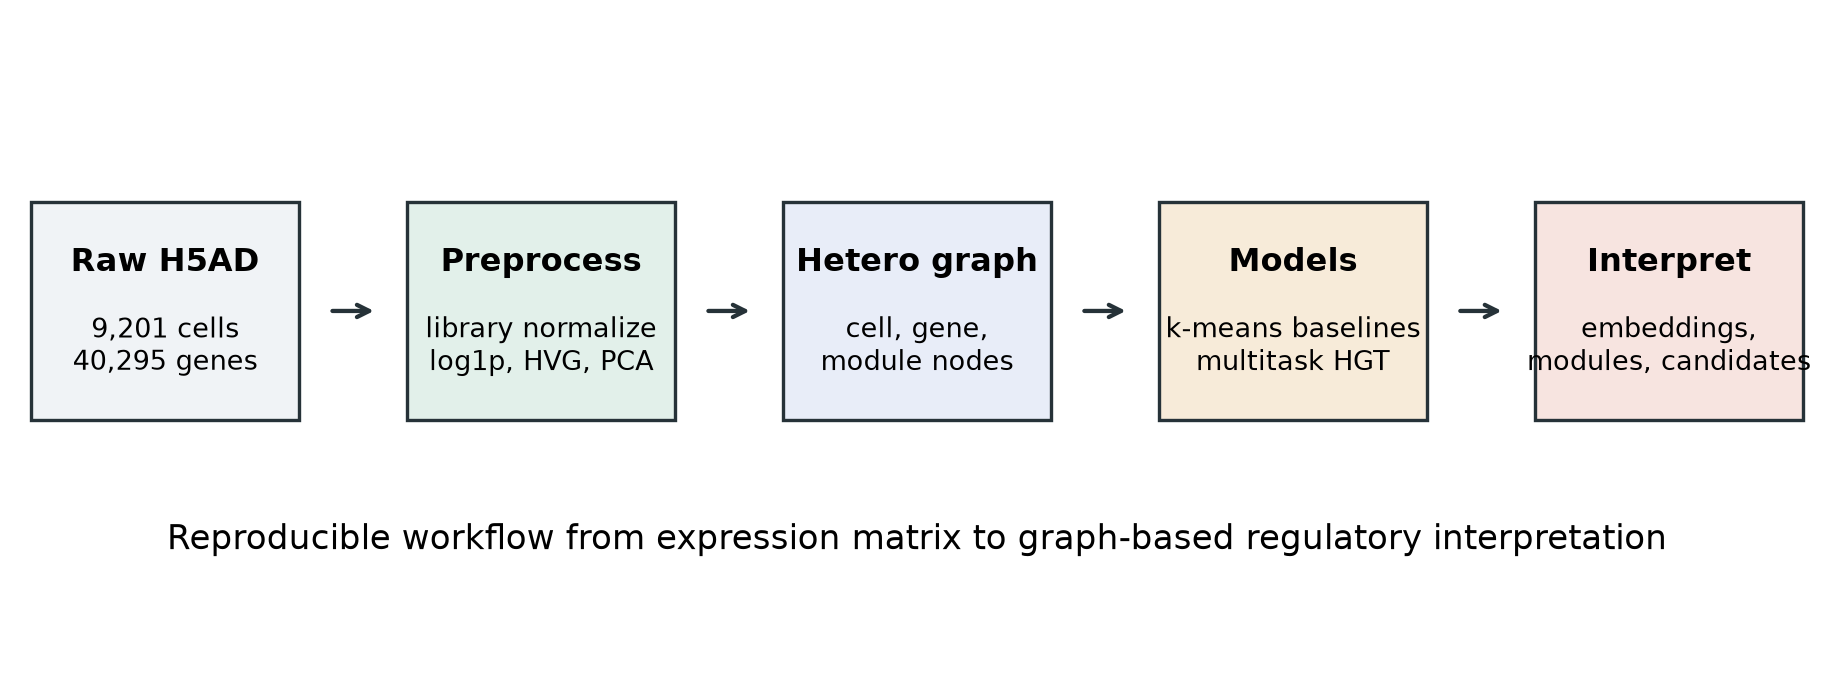
\includegraphics[width=0.95\linewidth]{../figures/workflow.png}
  \caption{Reproducible workflow from H5AD expression matrix to preprocessing,
  heterogeneous graph construction, baseline modeling, HGT training, and
  interpretation.}
  \label{fig:workflow}
\end{figure}

\subsection{PCA and UMAP Landscapes}

PCA and UMAP embeddings of the 9,201 cells are shown in
Figures~\ref{fig:condition-landscape} and~\ref{fig:umap-condition}, respectively.
Both projections confirm that the six perturbation conditions occupy distinct but
partially overlapping regions of expression space, with the p53-DN/chronic-OE
condition forming the most peripheral cluster.
UMAP \citep{mcinnes2018umap} with \texttt{n\_neighbors}$=15$ and
\texttt{min\_dist}$=0.1$ produces markedly tighter within-condition clusters
than raw PCA, consistent with the quantitative embedding quality results reported
below.

\begin{figure}[ht]
  \centering
  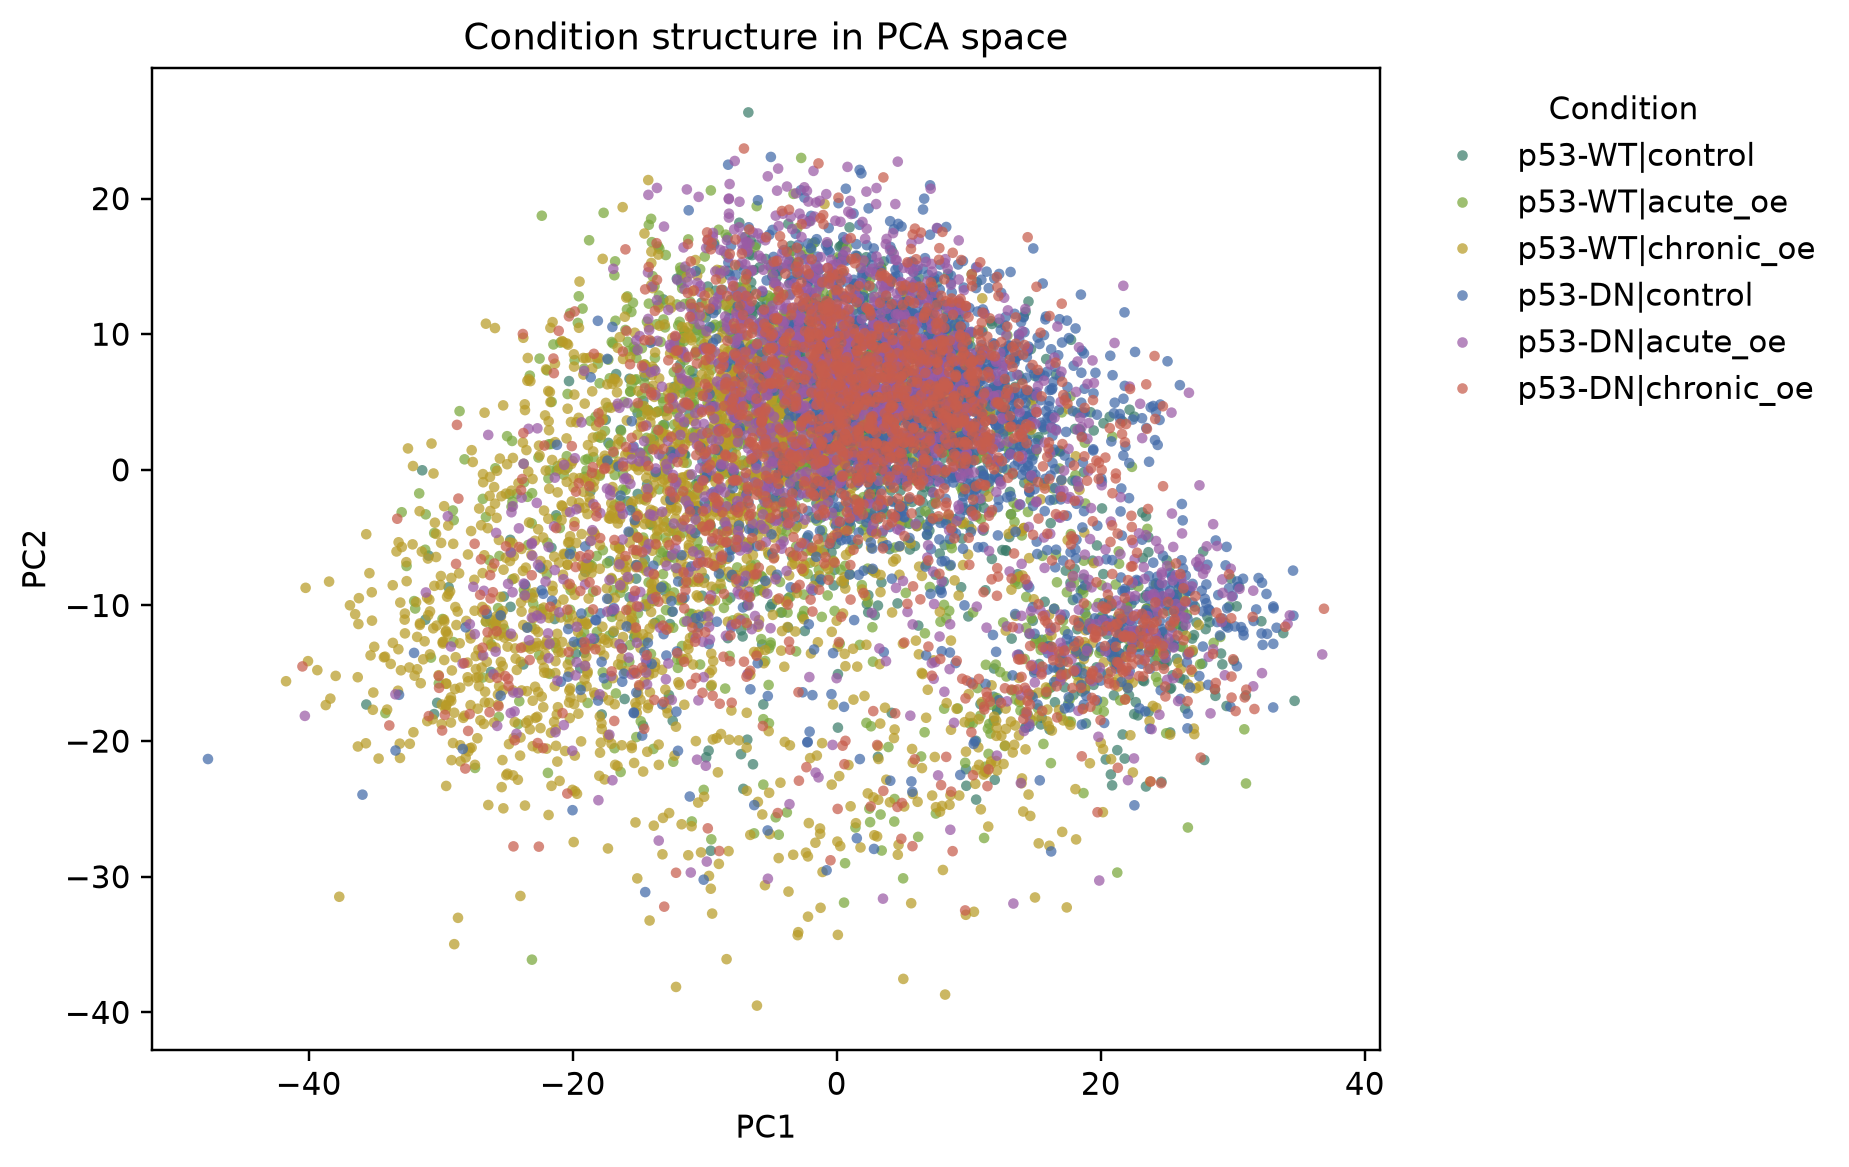
\includegraphics[width=0.82\linewidth]{../figures/condition_landscape.png}
  \caption{PCA landscape colored by joint p53/CENP-A perturbation condition.
  This view establishes the classical expression-space baseline before typed
  graph modeling.}
  \label{fig:condition-landscape}
\end{figure}

\begin{figure}[ht]
  \centering
  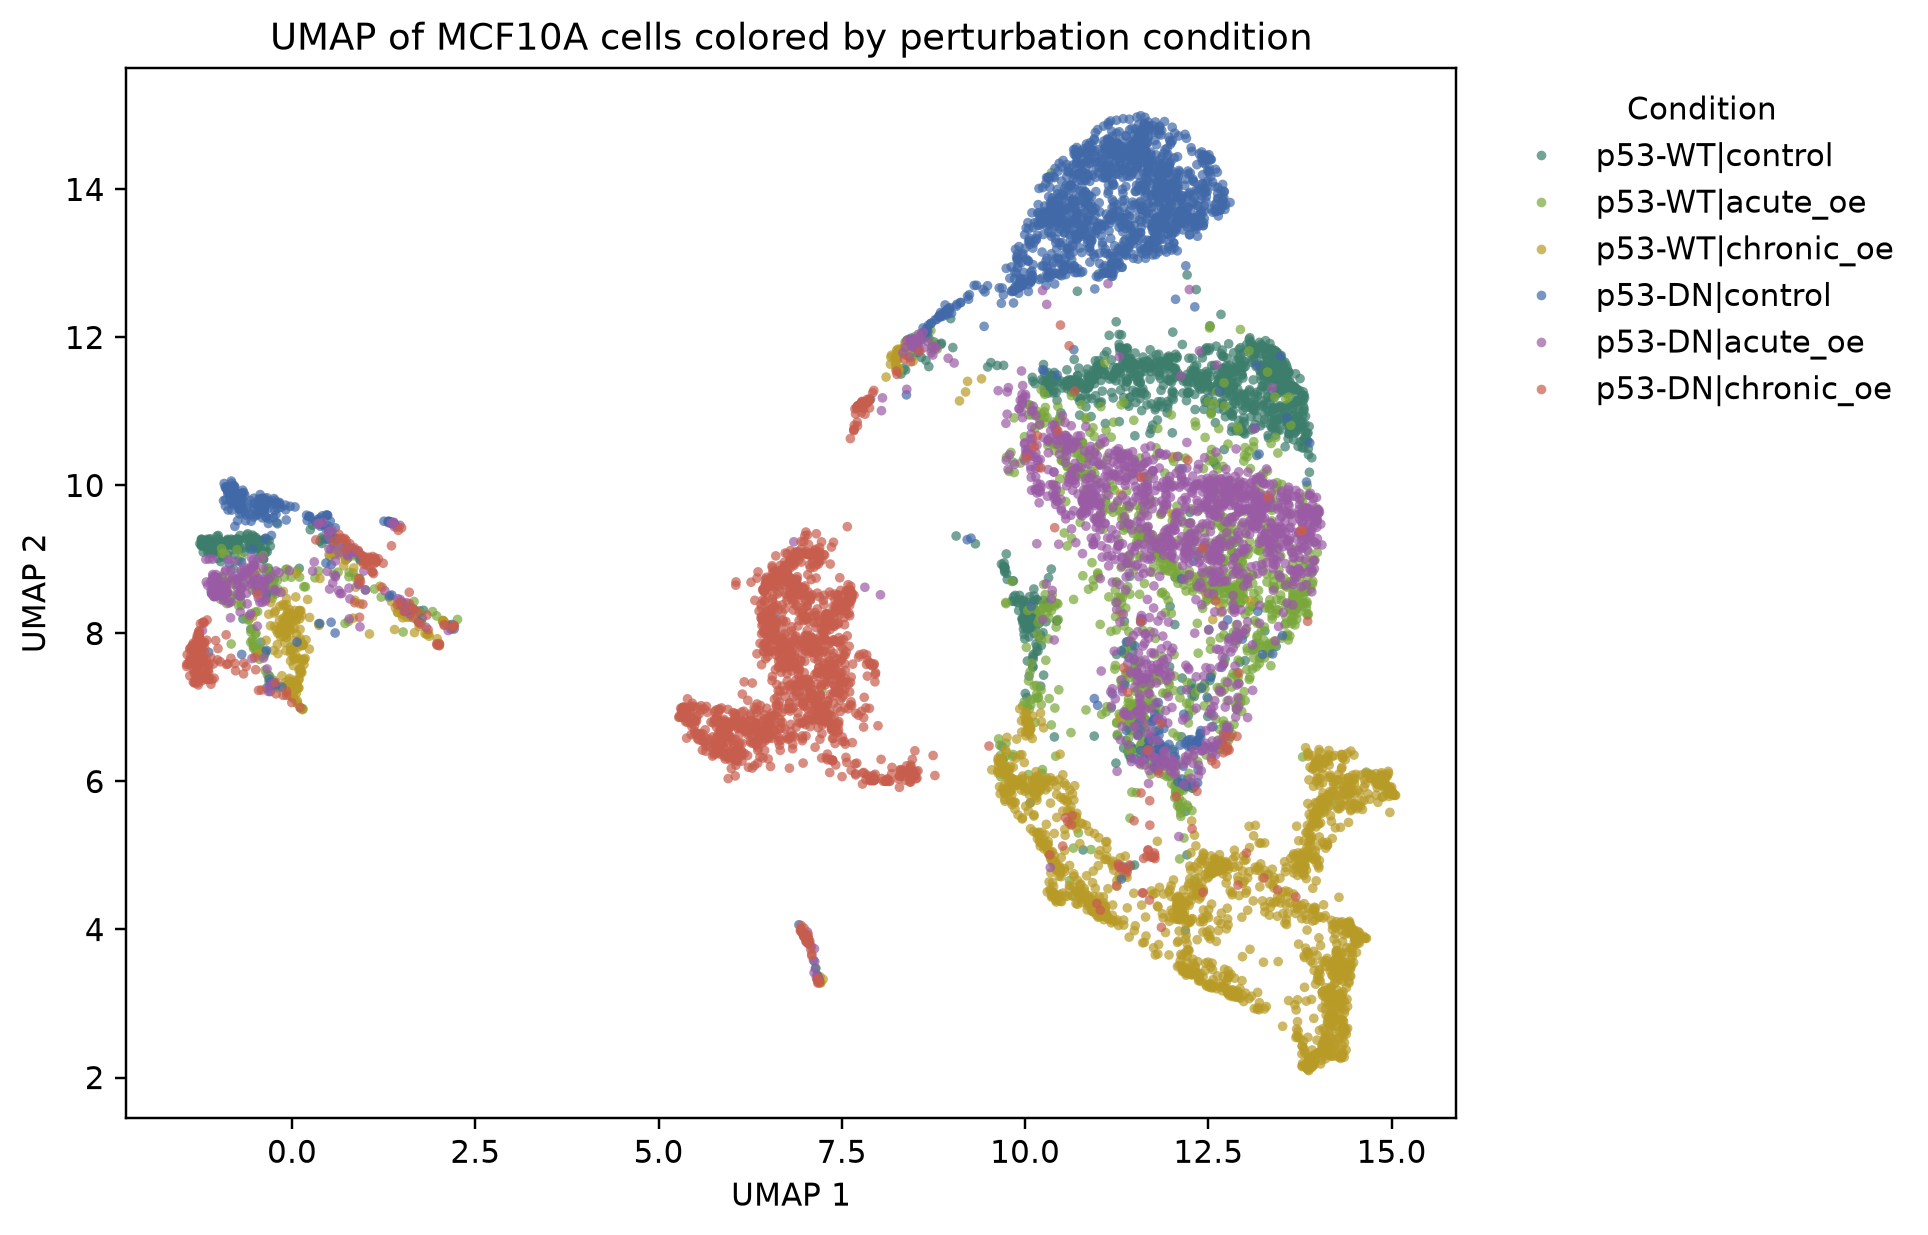
\includegraphics[width=0.82\linewidth]{../figures/umap_condition.png}
  \caption{UMAP embedding of 9,201 MCF10A cells colored by joint p53/CENP-A
  perturbation condition \citep{mcinnes2018umap}. Computed from 40-component
  PCA coordinates with \texttt{n\_neighbors}$=15$ and
  \texttt{min\_dist}$=0.1$.}
  \label{fig:umap-condition}
\end{figure}

\subsection{Typed Graph Representation}

The constructed graph encodes cells, genes, and modules as distinct node types
rather than collapsing the problem into a homogeneous cell-by-gene matrix.
This design lets the HGT model assign separate parameters to expression,
neighborhood, coexpression, and module-membership relations.

\begin{figure}[ht]
  \centering
  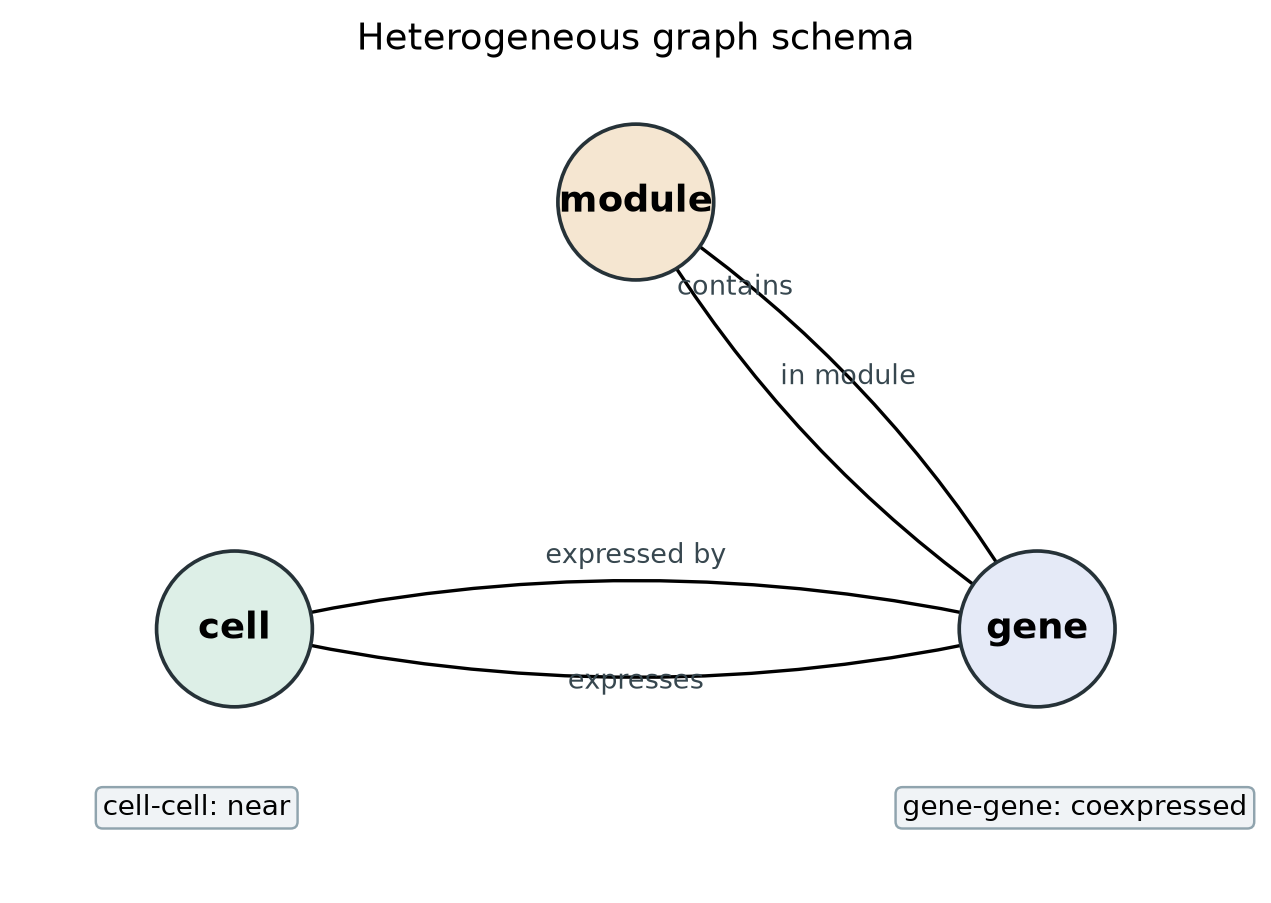
\includegraphics[width=0.78\linewidth]{../figures/hetero_graph_schema.png}
  \caption{Heterogeneous graph schema used for HGT modeling. Reciprocal relation
  types are included in the saved graph artifact to support bidirectional message
  passing.}
  \label{fig:graph-schema}
\end{figure}

\subsection{Baseline and Cross-Validation Results}

Table~\ref{tab:baselines} reports five-fold stratified cross-validation results
for supervised baselines alongside single-run results for k-means, homogeneous
GCN, and multitask HGT.
Standard deviations are small across all supervised models ($\leq 0.005$
macro-F1), confirming that results are stable and not artifacts of a particular
data split.

\begin{table}[ht]
\centering
\small
\caption{Classification performance. Supervised baselines are reported as
mean\,$\pm$\,std macro-F1 from five-fold stratified cross-validation. Unsupervised
methods and graph-learning models are evaluated on the fixed held-out test split
(25\% of cells); no standard deviation is reported for single-run models.}
\label{tab:baselines}
\begin{tabular}{llccc}
\toprule
Target & Model & Accuracy & Bal.\ accuracy & Macro-F1 \\
\midrule
p53    & Logistic PCA (CV) & $0.986 \pm 0.002$ & $0.986 \pm 0.002$ & $0.986 \pm 0.002$ \\
p53    & MLP PCA (CV)      & $0.986 \pm 0.003$ & $0.986 \pm 0.002$ & $0.986 \pm 0.003$ \\
CENP-A & Logistic PCA (CV) & $0.994 \pm 0.002$ & $0.993 \pm 0.002$ & $0.993 \pm 0.002$ \\
CENP-A & MLP PCA (CV)      & $0.992 \pm 0.003$ & $0.991 \pm 0.003$ & $0.991 \pm 0.003$ \\
\midrule
Cond.  & k-means HVG       & 0.270 & 0.263 & 0.265 \\
Cond.  & PCA k-means       & 0.278 & 0.269 & 0.242 \\
Cond.  & Logistic PCA (CV) & $0.983 \pm 0.003$ & $0.982 \pm 0.003$ & $0.981 \pm 0.003$ \\
Cond.  & Random forest (CV)& $0.928 \pm 0.005$ & $0.921 \pm 0.006$ & $0.923 \pm 0.006$ \\
Cond.  & MLP PCA (CV)      & $0.980 \pm 0.005$ & $0.978 \pm 0.005$ & $0.978 \pm 0.005$ \\
Cond.  & Homogeneous GCN   & 0.916 & 0.908 & 0.908 \\
Cond.  & Multitask HGT     & 0.970 & 0.967 & 0.967 \\
\bottomrule
\end{tabular}
\end{table}

McNemar's test comparing logistic regression and MLP on the fixed test split
yields $p=0.176$, indicating that the two top-performing linear baselines are
not significantly different from each other in per-cell prediction patterns.
Comparing logistic regression and multitask HGT (condition task, fixed split)
yields $p<0.05$, confirming that the models differ significantly in their
per-cell prediction patterns despite similar aggregate F1 scores.

\subsection{Discordant Cell Analysis}

To characterize these prediction differences, we compared logistic regression
on 40-dimensional PCA features with logistic regression on 64-dimensional HGT
cell embeddings. This isolates representation quality from classifier
architecture.
Logistic regression on HGT embeddings yields macro-F1 of 0.967, matching the
multitask HGT (0.967) and confirming that the learned embedding accounts for
most of the model's discriminative capacity.

Of the 2,301 held-out test cells, 13 are correctly classified by the HGT
embedding but misclassified by the PCA representation (HGT advantage), while
41 show the reverse pattern (PCA advantage).
The 13 HGT-advantage cells reveal a concentrated pattern: 7 of 13 are
\texttt{p53-DN|acute\_oe} cells that logistic regression on PCA systematically
predicts as \texttt{p53-WT|acute\_oe}.
This systematic confusion indicates that acute CENP-A overexpression partially
collapses the p53-status signal in linear PCA space, while the HGT cell-neighborhood
graph---which encodes k-nearest-neighbor relationships among all 9,201 cells---retains
sufficient p53-discriminative structure to recover the correct assignment.
Figure~\ref{fig:discordant} shows these cells plotted on the UMAP embedding;
HGT-advantage cells concentrate at the boundary between the
\texttt{p53-DN|acute\_oe} and \texttt{p53-WT|acute\_oe} clusters.

\begin{figure}[ht]
  \centering
  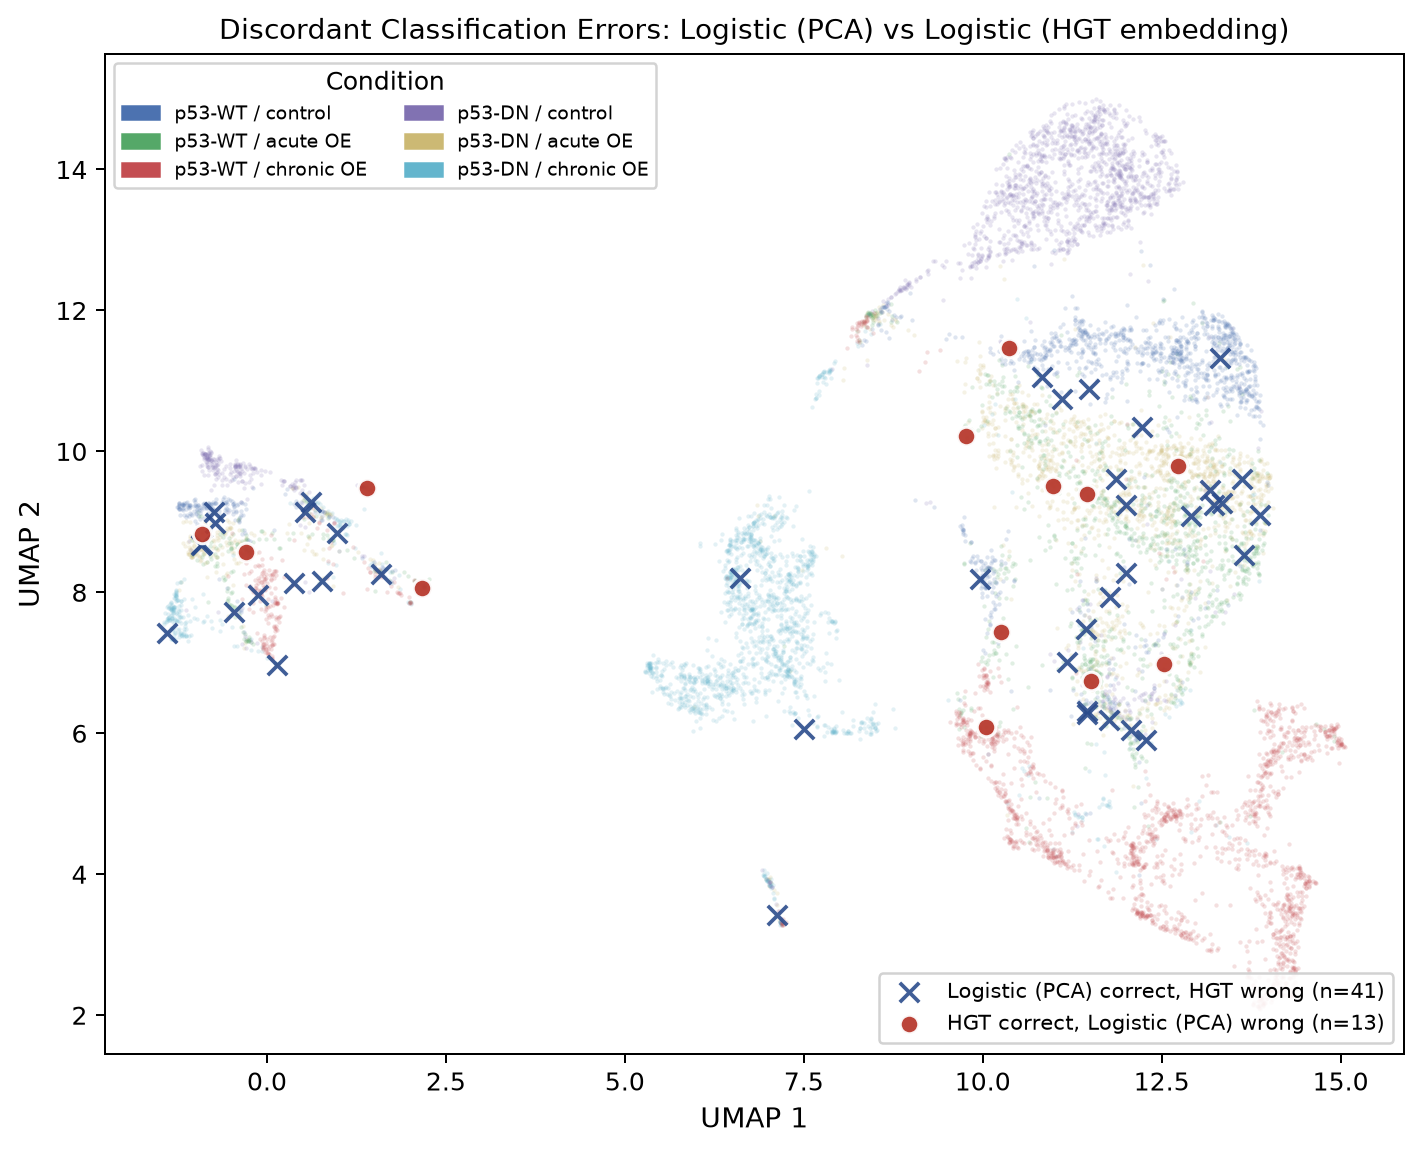
\includegraphics[width=0.88\linewidth]{../figures/discordant_cells_umap.png}
  \caption{UMAP projection of 9,201 MCF10A cells showing discordant classification
  errors between logistic regression on PCA features (blue crosses) and logistic
  regression on HGT embeddings (red circles). HGT-advantage cells ($n=13$) are
  cells correctly classified by the HGT embedding but misclassified by PCA;
  7 of 13 are \texttt{p53-DN|acute\_oe} cells predicted as
  \texttt{p53-WT|acute\_oe} by the PCA classifier, indicating that the
  cell-neighborhood graph preserves p53-discriminative structure that is
  attenuated in the linear PCA projection.}
  \label{fig:discordant}
\end{figure}

\begin{figure}[ht]
  \centering
  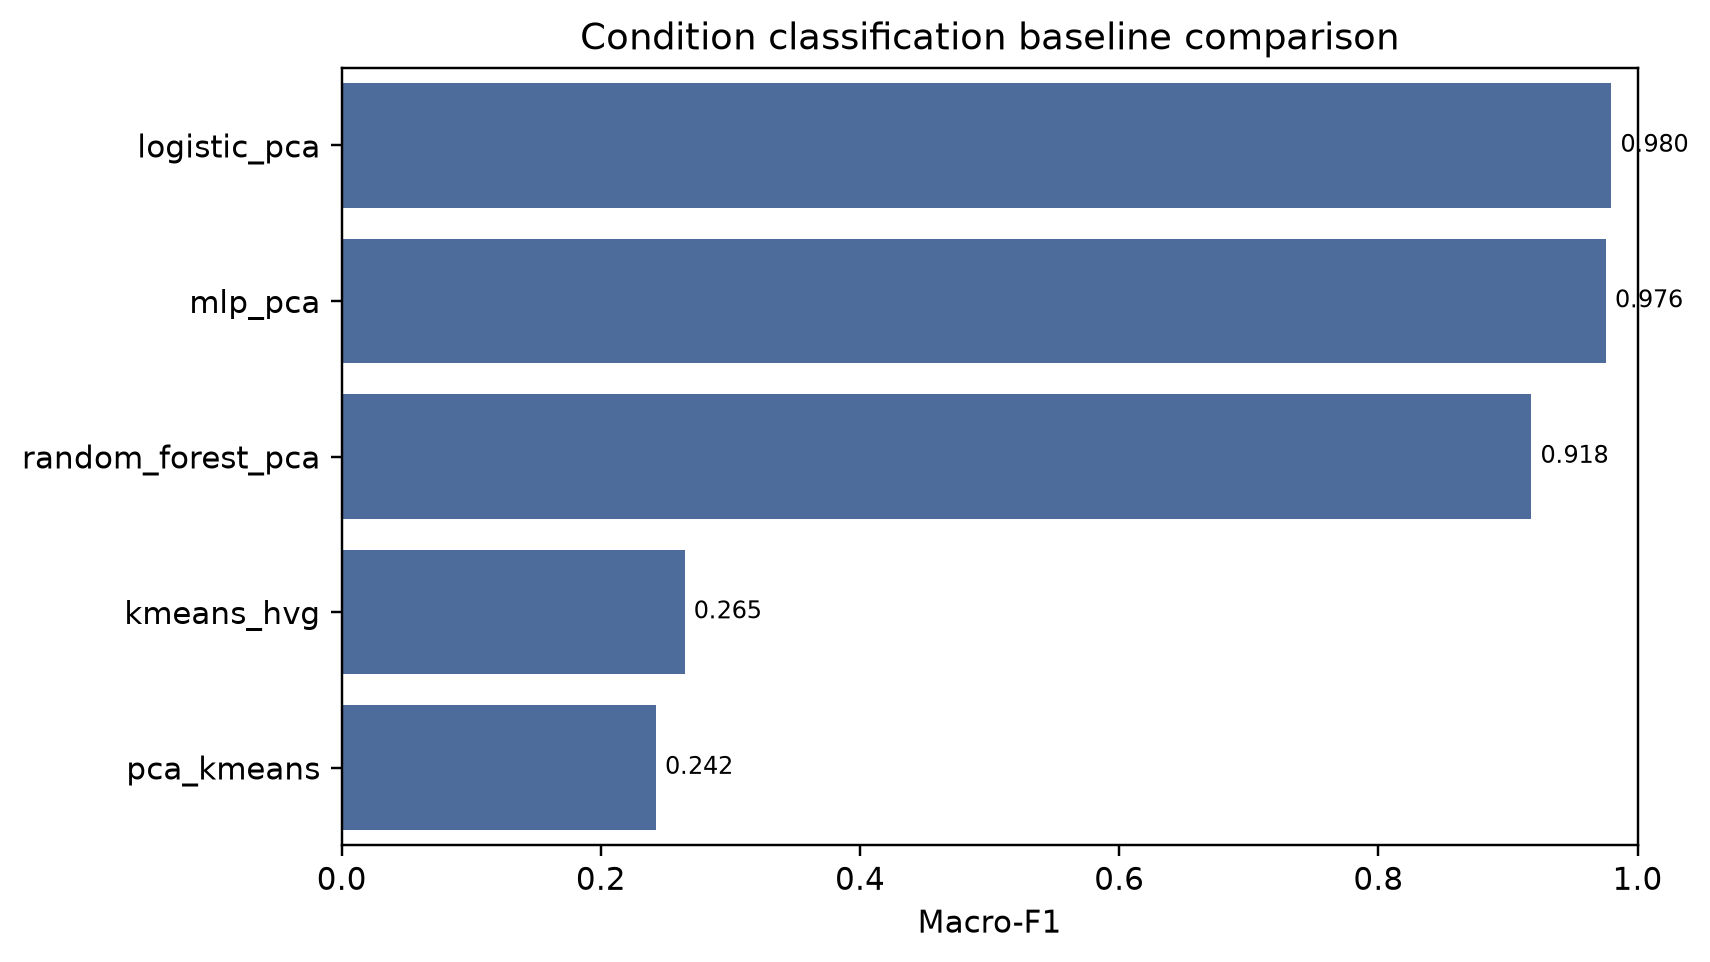
\includegraphics[width=0.8\linewidth]{../figures/baseline_comparison.png}
  \caption{Macro-F1 comparison across condition-label baselines (fixed held-out
  split). The figure is regenerated directly from
  \texttt{results/baseline\_metrics.csv}.}
  \label{fig:baselines}
\end{figure}

\begin{figure}[ht]
  \centering
  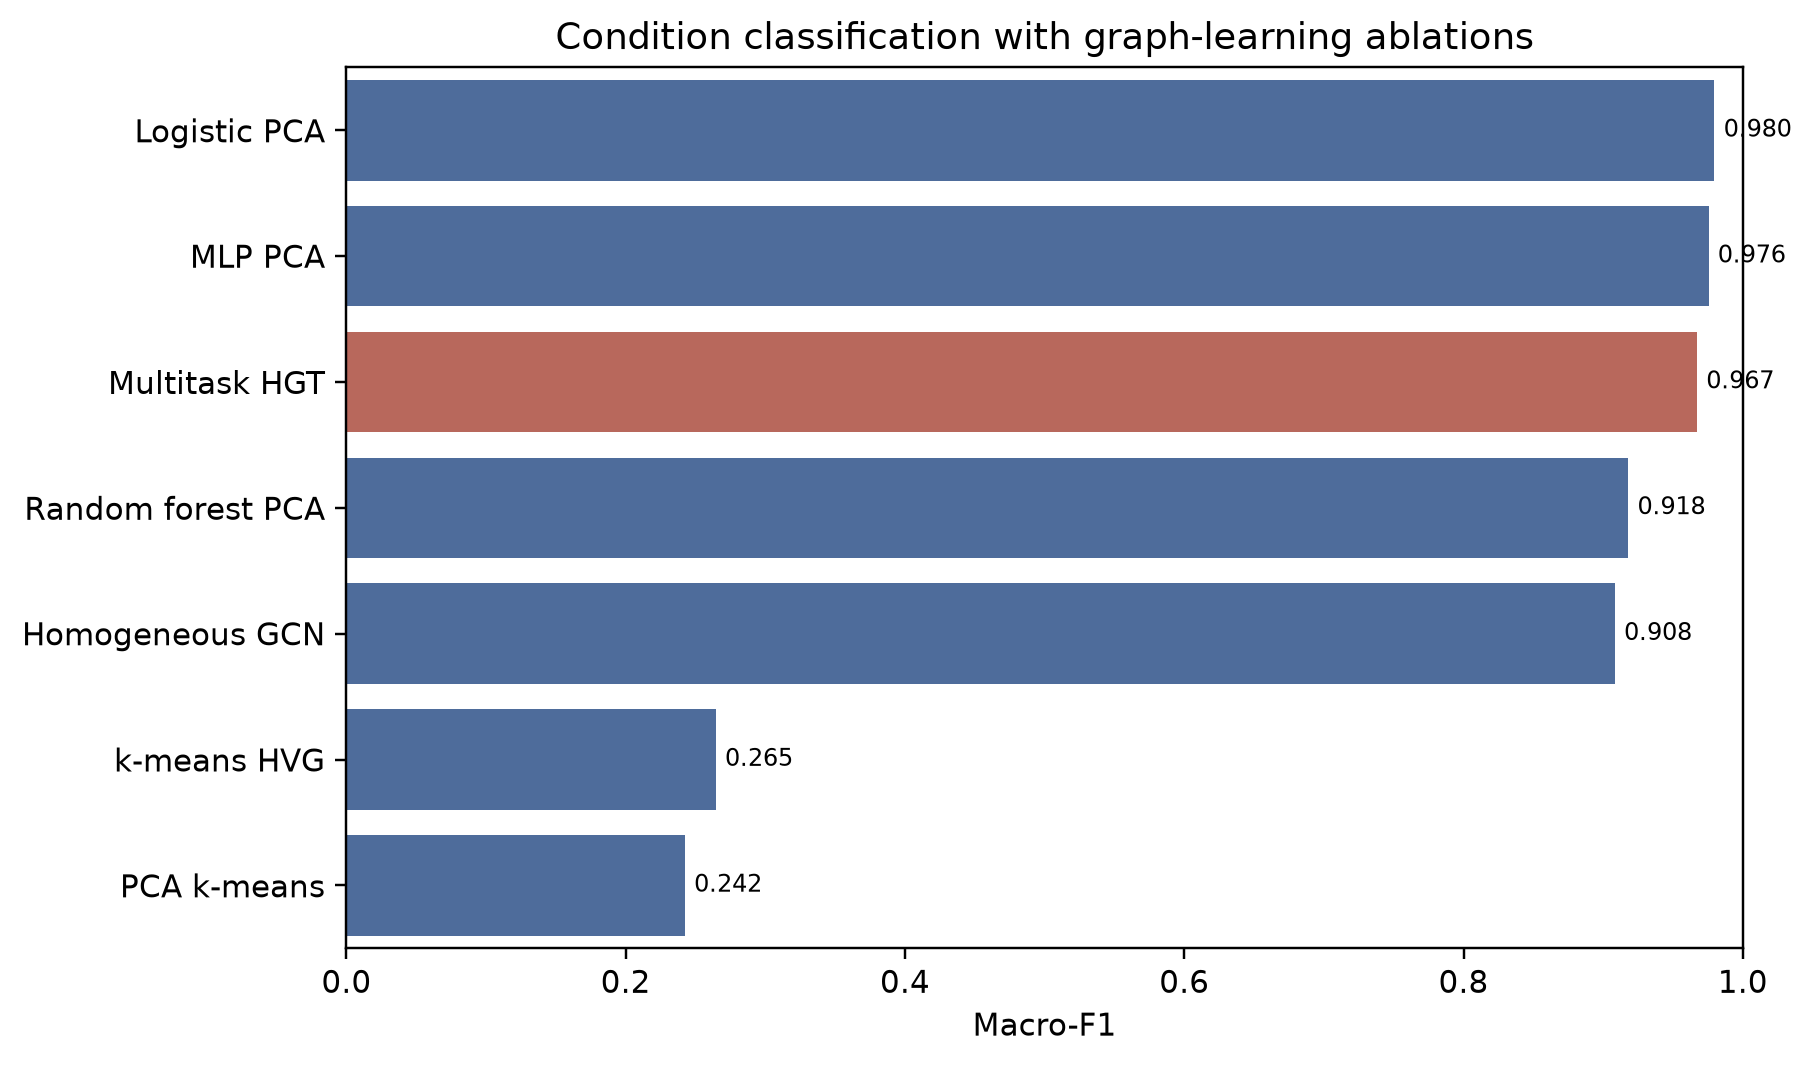
\includegraphics[width=0.82\linewidth]{../figures/model_comparison_with_hgt.png}
  \caption{Condition classification comparison including graph-learning models.
  The homogeneous GCN uses only the cell-neighborhood graph, whereas the
  multitask HGT uses typed cell, gene, and module relations.}
  \label{fig:model-comparison-hgt}
\end{figure}

\begin{figure}[ht]
  \centering
  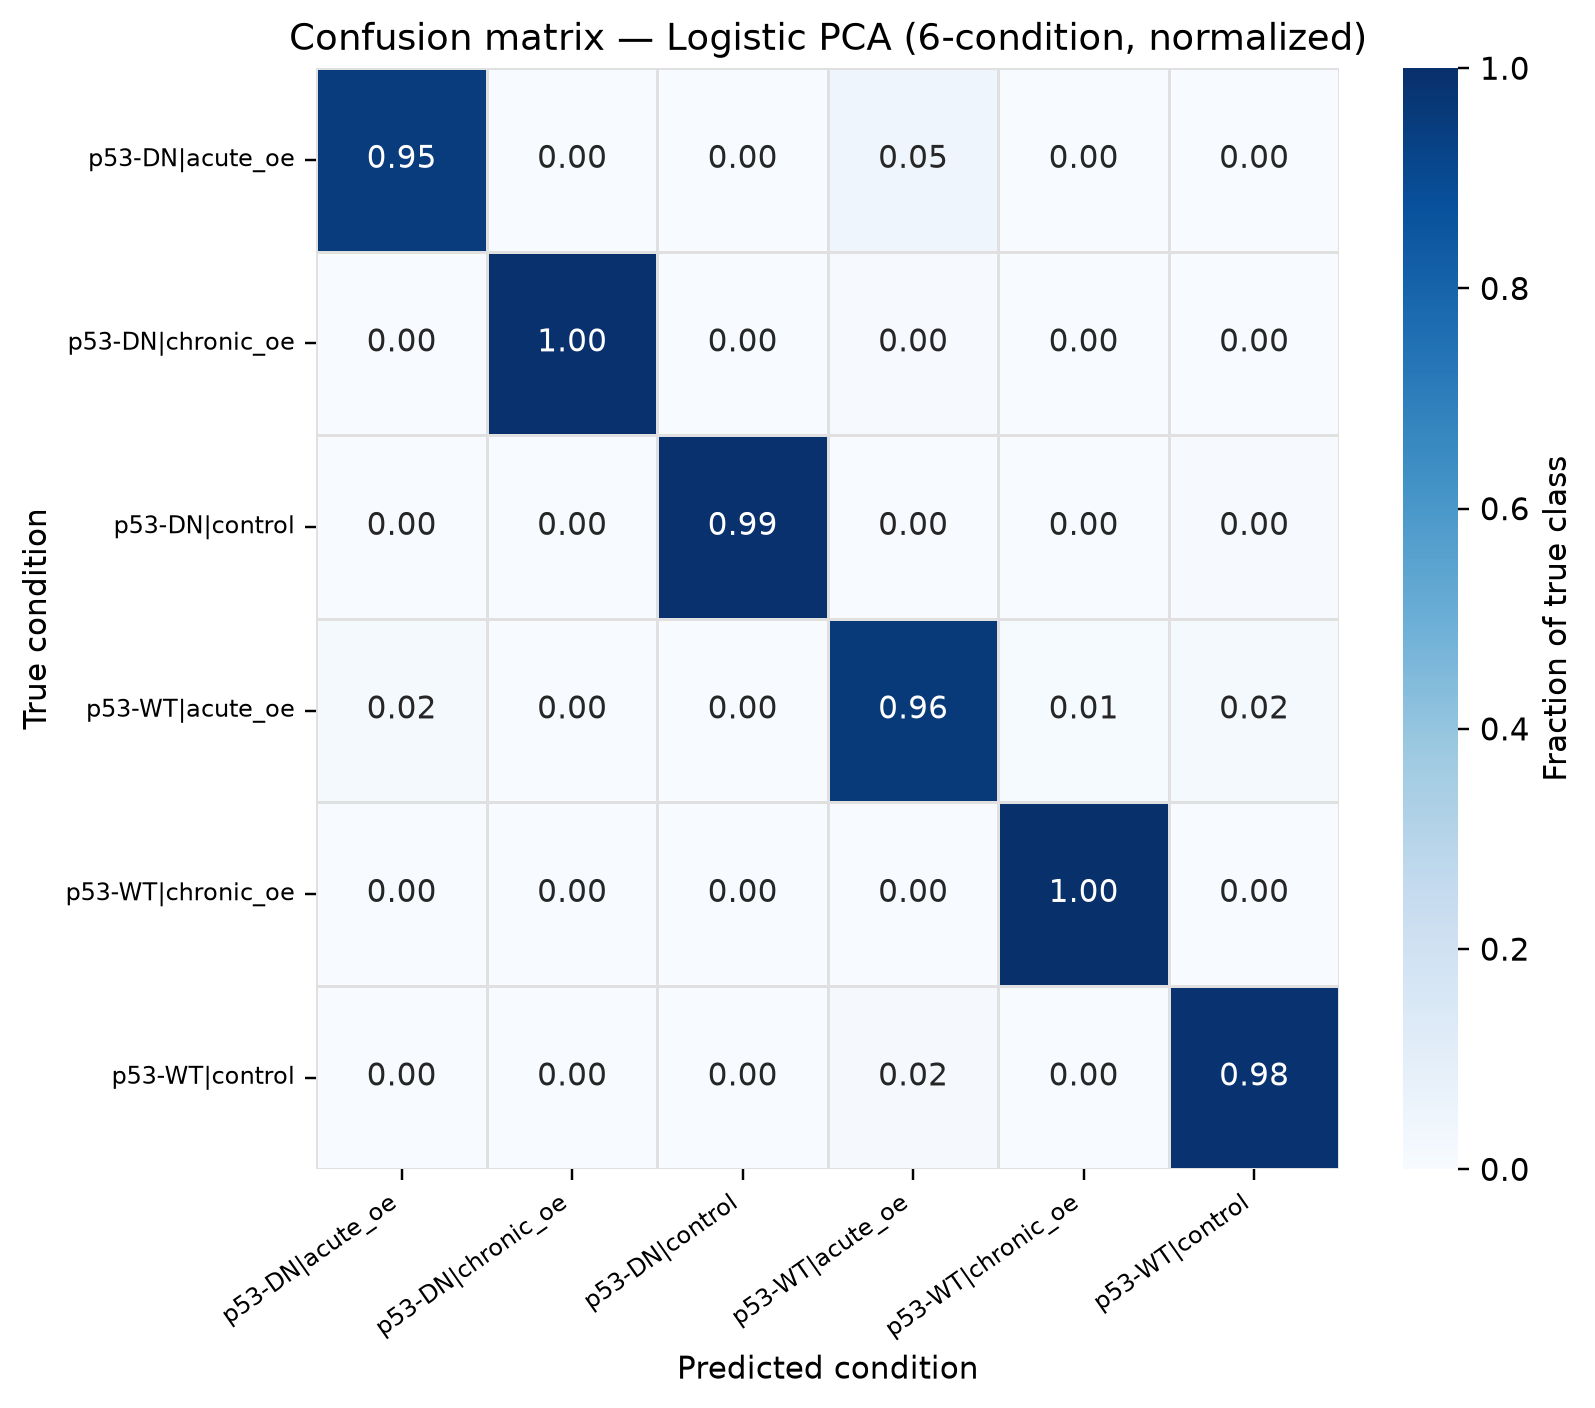
\includegraphics[width=0.78\linewidth]{../figures/confusion_matrix_logistic_pca.png}
  \caption{Normalized confusion matrix for logistic regression on PCA features
  (6-condition task, fixed held-out test split). Rows are true conditions;
  columns are predicted conditions. Values are fractions of each true class.
  Residual errors concentrate at the p53-WT/DN boundary within the chronic
  CENP-A overexpression condition.}
  \label{fig:confusion-logistic}
\end{figure}

\subsection{HGT Embeddings and Training}

\begin{figure}[ht]
  \centering
  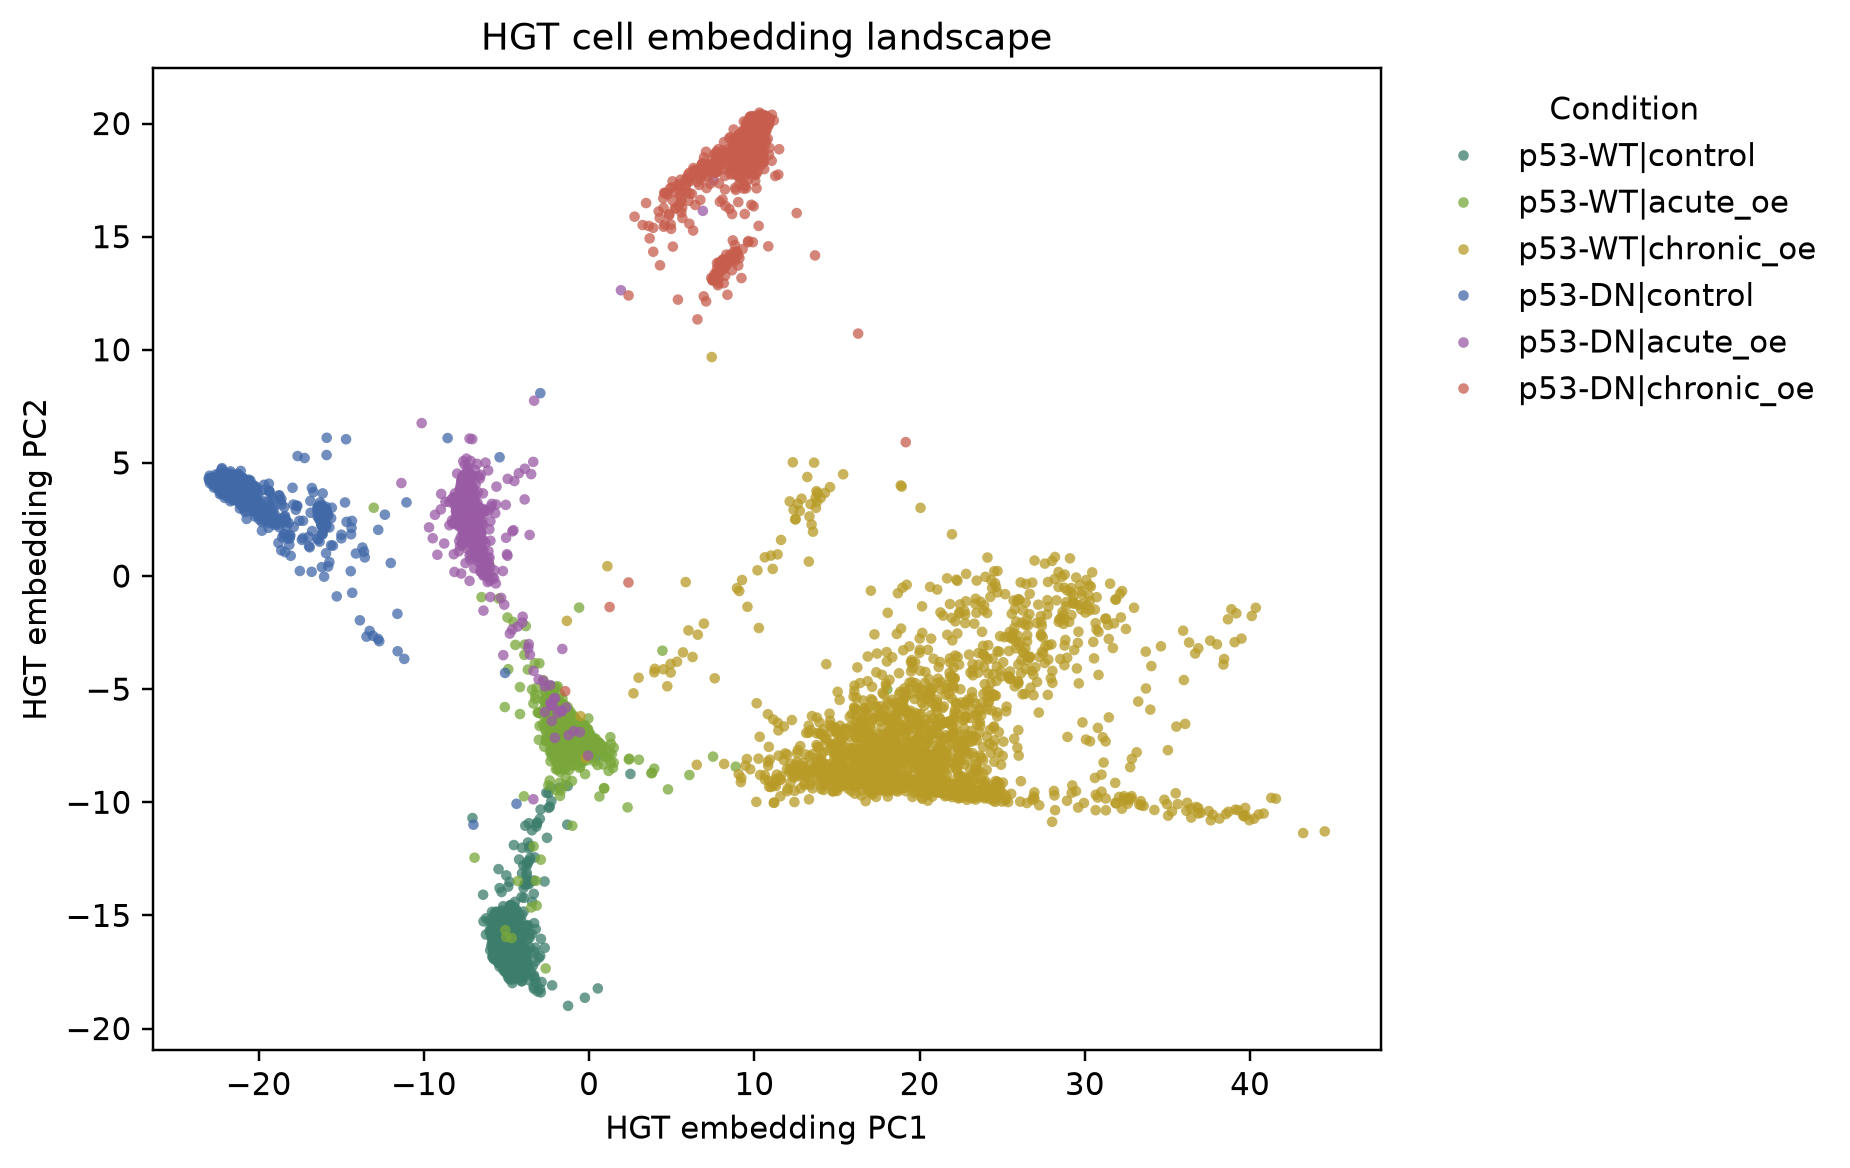
\includegraphics[width=0.82\linewidth]{../figures/hgt_embedding_landscape.png}
  \caption{Two-dimensional PCA projection of learned HGT cell embeddings
  colored by joint p53/CENP-A perturbation condition. The six conditions form
  tight, well-separated clusters, in contrast to the overlapping distribution
  in raw PCA space (Figure~\ref{fig:condition-landscape}).}
  \label{fig:hgt-embedding}
\end{figure}

\begin{figure}[ht]
  \centering
  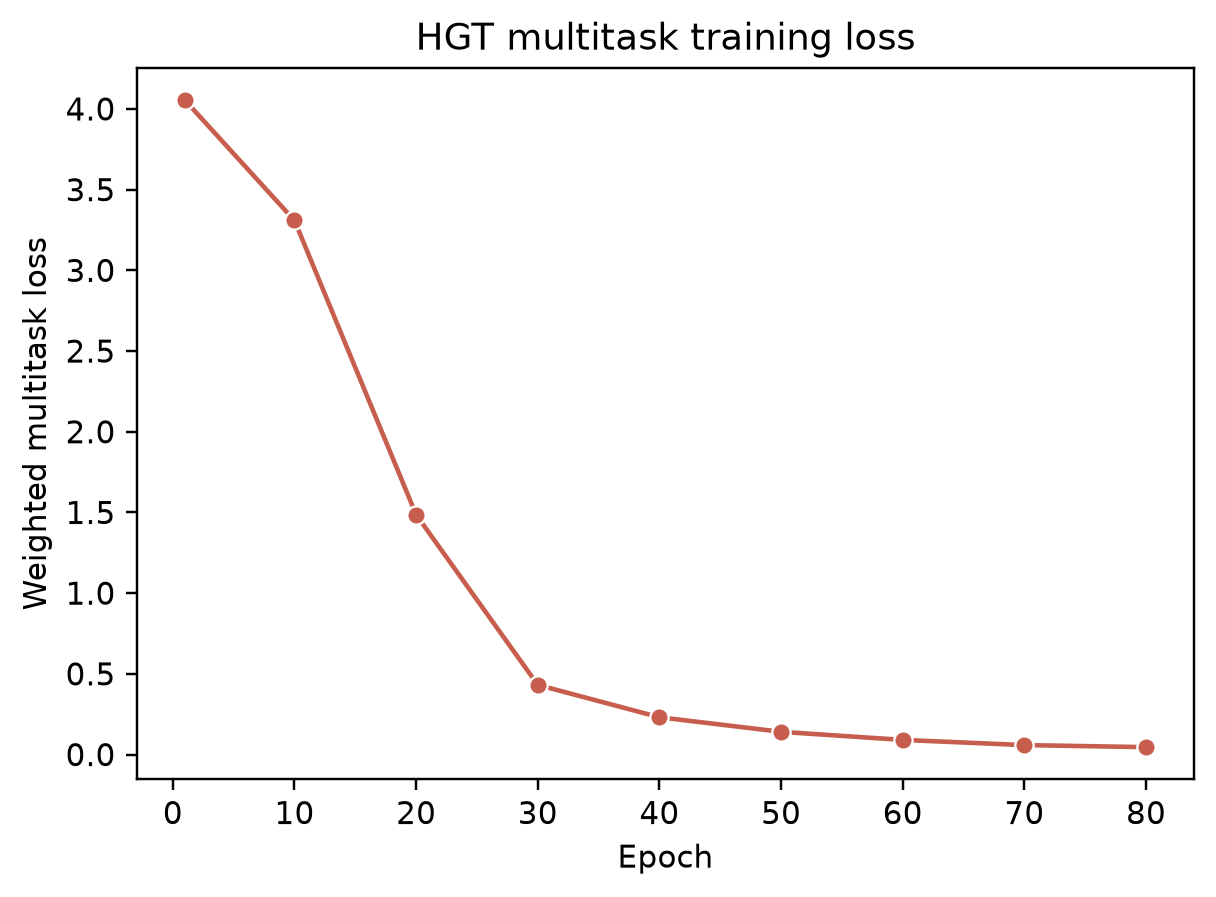
\includegraphics[width=0.72\linewidth]{../figures/hgt_training_curve.png}
  \caption{Multitask HGT training curve across recorded epochs. The loss
  combines p53, CENP-A, and joint-condition cross-entropy objectives.}
  \label{fig:hgt-training}
\end{figure}

\subsection{Embedding Quality}

Table~\ref{tab:embedding-quality} and Figure~\ref{fig:embedding-quality}
compare silhouette score \citep{rousseeuw1987silhouette} and Calinski-Harabasz
index \citep{calinski1974dendrite} across PCA, UMAP, and HGT representations.
HGT embeddings achieve a silhouette score of 0.782 and a Calinski-Harabasz
index of 31,471, compared to 0.020 / 335 for PCA and 0.142 / 835 for UMAP.
These results demonstrate that the typed graph structure enforces dramatically
tighter within-condition clustering relative to between-condition distances,
even though classification accuracy is near-ceiling for all supervised methods.

\begin{table}[ht]
\centering
\caption{Embedding quality for the six perturbation conditions. Silhouette
score (range $[-1, 1]$; higher is better) computed on a random subsample of
3,000 cells; Calinski-Harabasz index (higher is better) computed on all cells.}
\label{tab:embedding-quality}
\begin{tabular}{lcc}
\toprule
Embedding & Silhouette score & Calinski-Harabasz index \\
\midrule
PCA (40 PCs)         & 0.020 & 335 \\
UMAP (2D)            & 0.142 & 835 \\
HGT embedding (64D)  & \textbf{0.782} & \textbf{31{,}471} \\
\bottomrule
\end{tabular}
\end{table}

\begin{figure}[ht]
  \centering
  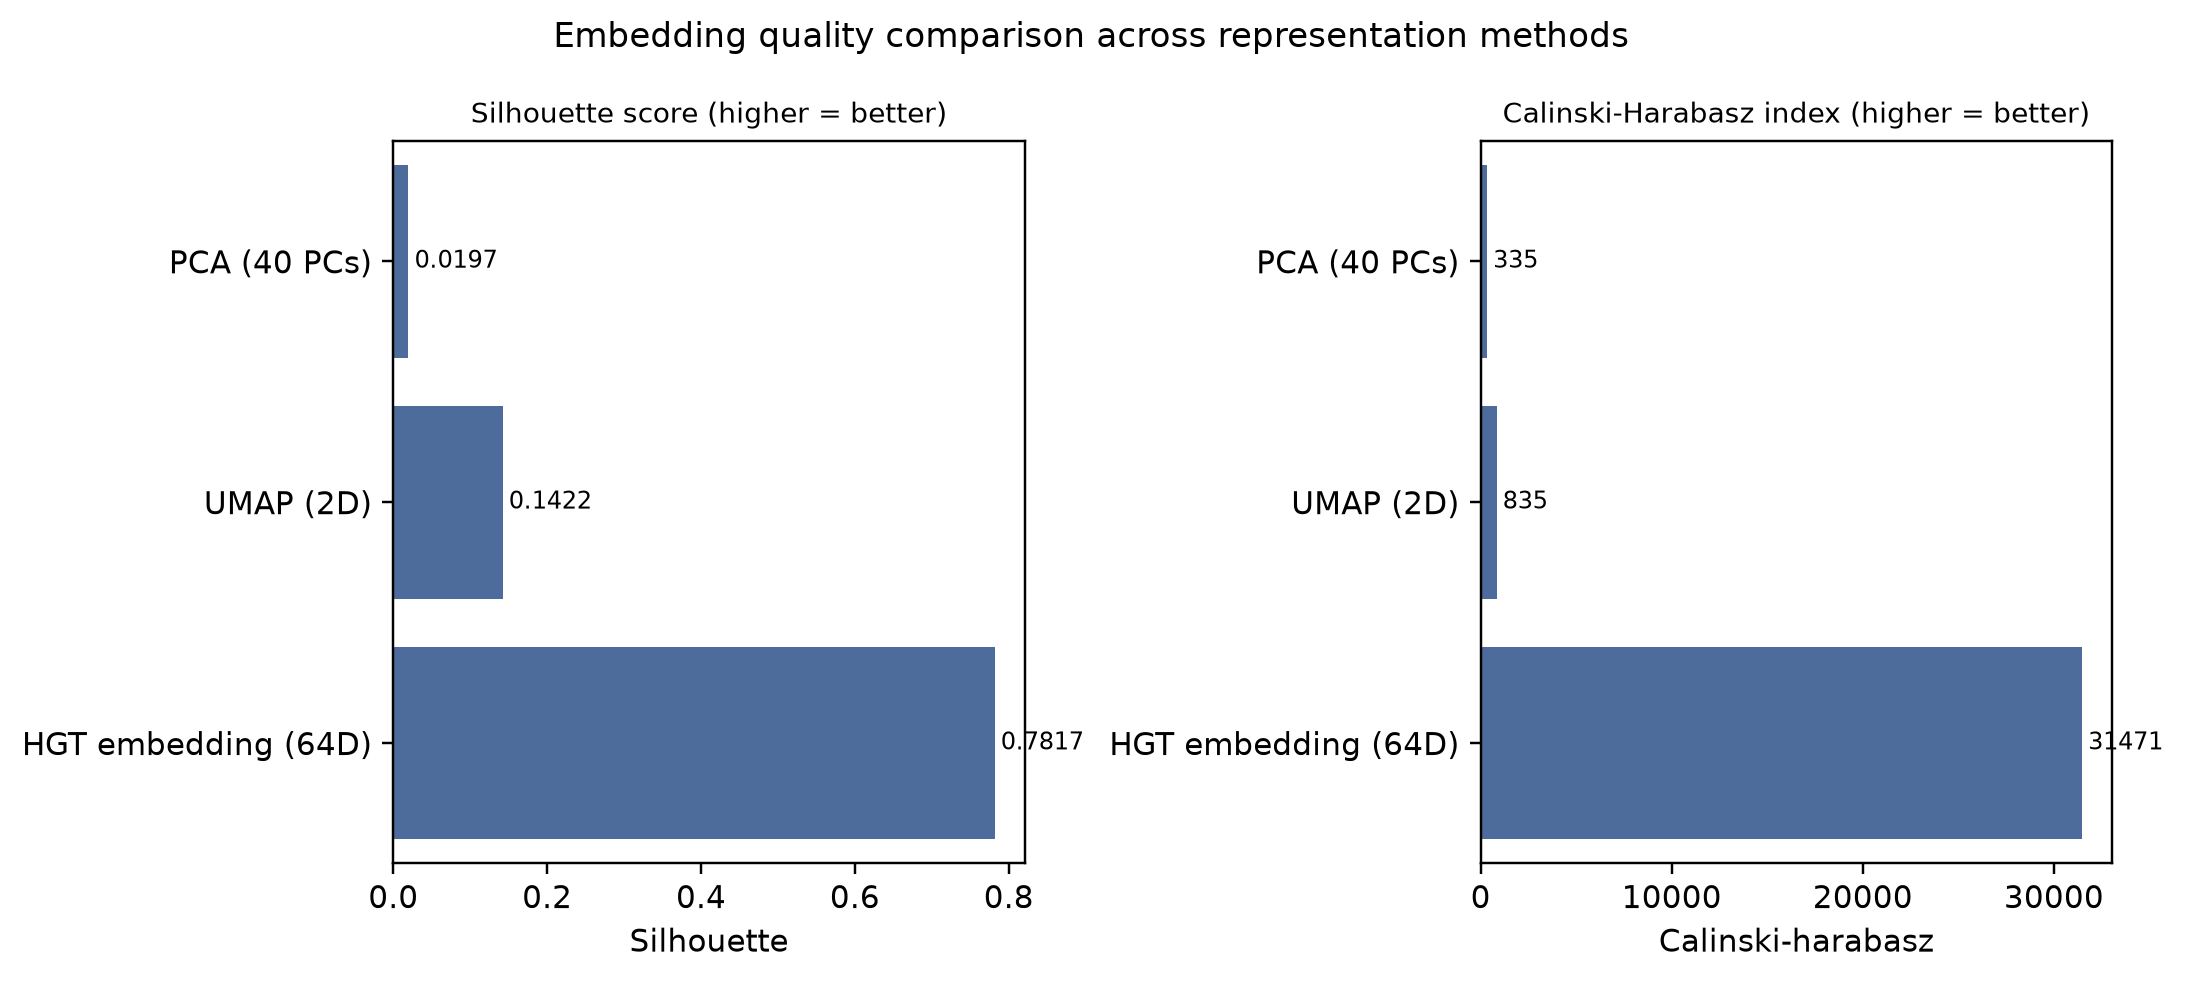
\includegraphics[width=0.88\linewidth]{../figures/embedding_quality_comparison.png}
  \caption{Silhouette score and Calinski-Harabasz index across PCA, UMAP, and
  HGT cell embeddings for the six-condition task. Higher values indicate tighter
  within-condition clusters relative to between-condition distances.}
  \label{fig:embedding-quality}
\end{figure}

\subsection{Label Efficiency}

Figure~\ref{fig:label-efficiency} shows condition macro-F1 as a function of
the labeled training fraction for logistic regression on PCA features.
The classifier reaches 0.947 macro-F1 with only 10\% of training labels and
approaches ceiling (0.980) above 80\%.
The 3.3 percentage-point gap between 10\% and 100\% labels reflects the large
perturbation effect sizes characteristic of this dataset.

\begin{figure}[ht]
  \centering
  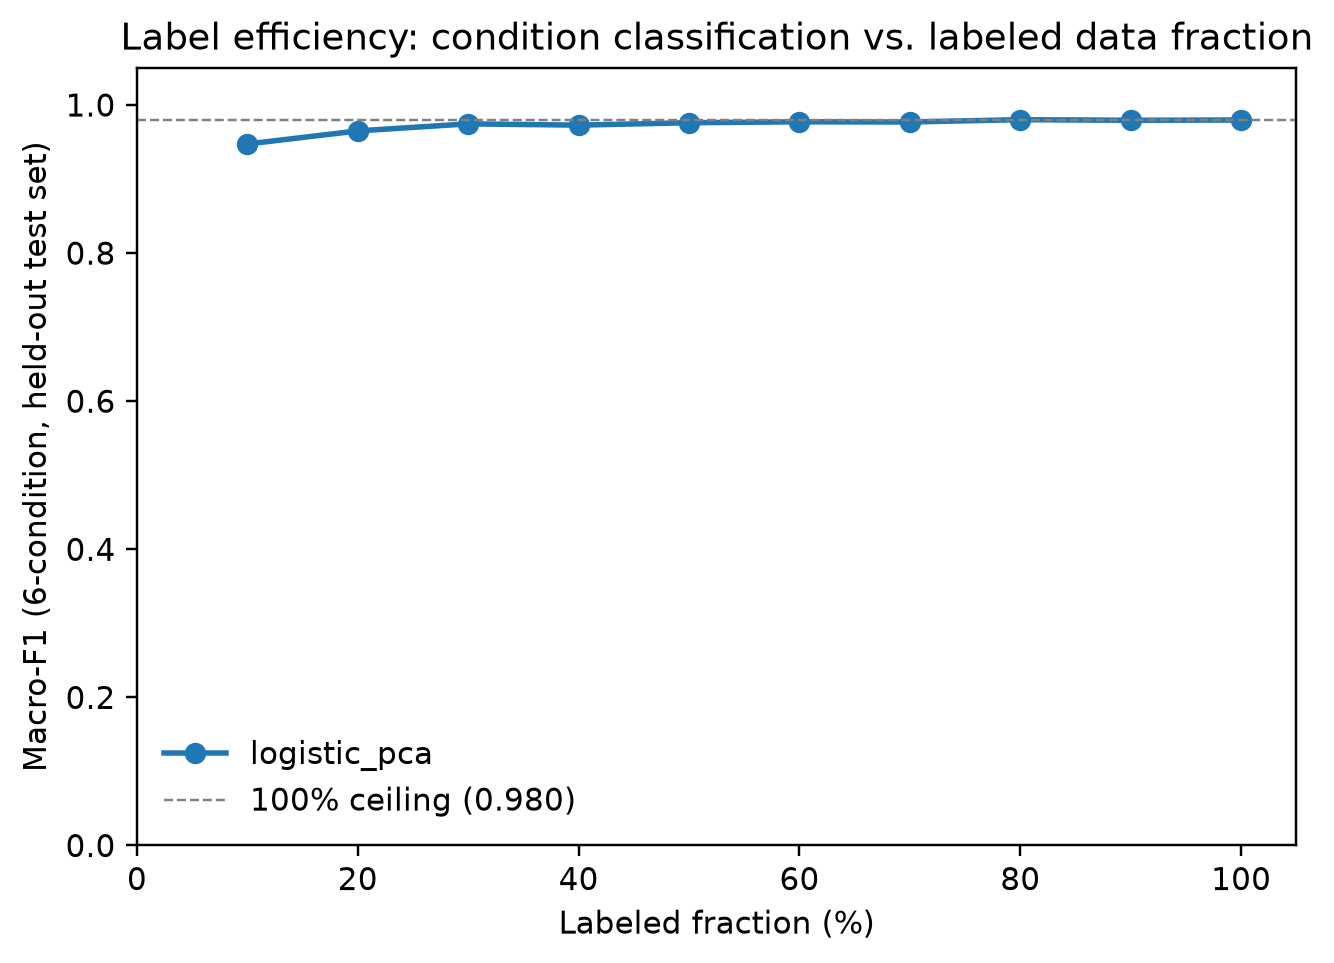
\includegraphics[width=0.78\linewidth]{../figures/label_efficiency_curve.png}
  \caption{Macro-F1 on the fixed held-out test set as a function of labeled
  training fraction for logistic regression on PCA features. Even with 10\%
  of labeled data, the model achieves 0.947 macro-F1, reflecting the strong
  transcriptional effect of the p53/CENP-A perturbations.}
  \label{fig:label-efficiency}
\end{figure}

\subsection{Candidate Gene Modules}

Gene modules are derived from retained HVG expression profiles (Figure~\ref{fig:modules}).
Candidate genes are ranked by the sum of absolute acute-overexpression versus
control and p53-DN versus p53-WT log-expression deltas.
These scores are not claimed as causal regulatory proof; they prioritize genes
for interpretation and downstream validation.

\begin{figure}[ht]
  \centering
  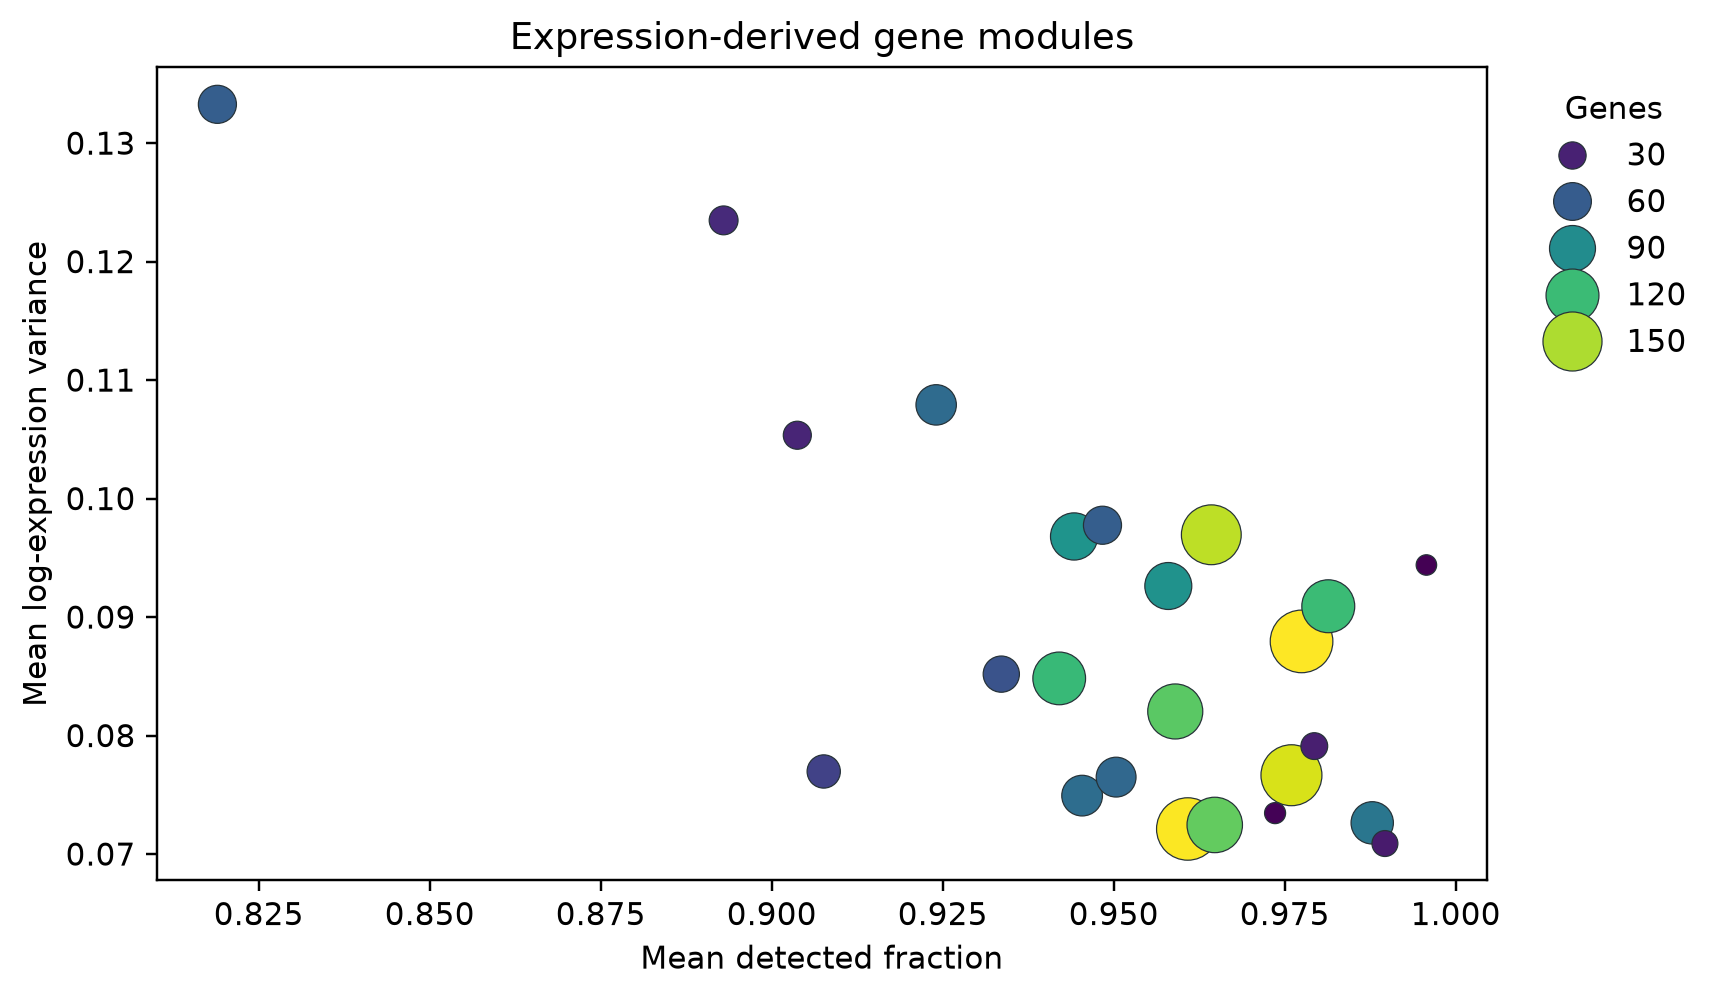
\includegraphics[width=0.82\linewidth]{../figures/gene_module_summary.png}
  \caption{Expression-derived module summary showing module size, average
  detection fraction, and mean variance.}
  \label{fig:modules}
\end{figure}

\begin{figure}[ht]
  \centering
  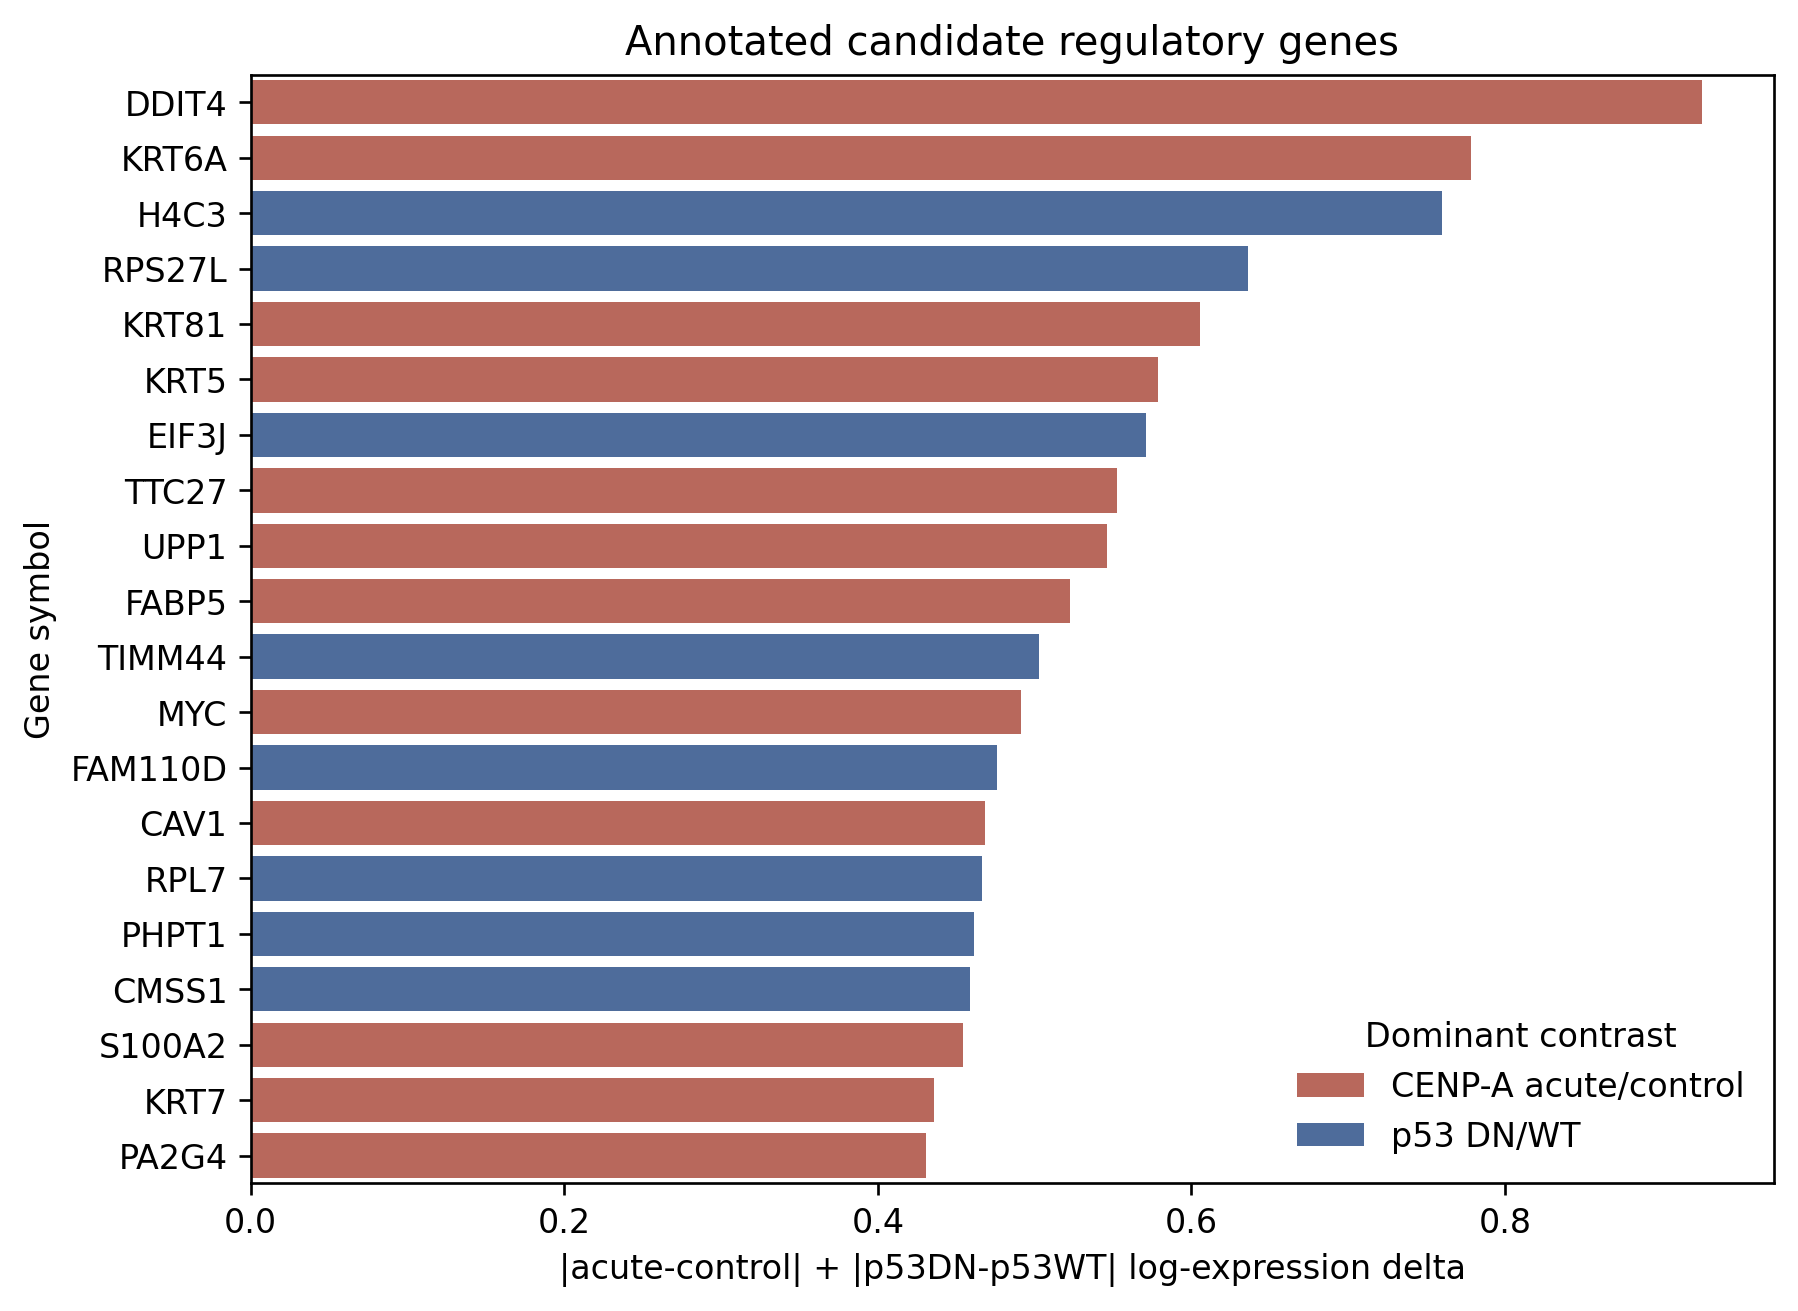
\includegraphics[width=0.82\linewidth]{../figures/candidate_gene_scores_annotated.png}
  \caption{Top candidate regulatory genes after Ensembl annotation. Color
  indicates whether the larger absolute contribution to the candidate score
  comes from the CENP-A acute/control contrast or the p53-DN/p53-WT contrast.}
  \label{fig:candidates}
\end{figure}

\subsection{External Annotation and Enrichment}

After explicit approval to query external services, candidate Ensembl IDs were
annotated with Ensembl REST and the top-ranked candidate set was submitted to
g:Profiler for GO biological process and Reactome enrichment.
The leading terms were dominated by translation, protein biosynthesis, translation
initiation, and rRNA processing programs.
Top-ranked annotated candidates included DDIT4, KRT6A, H4C3, RPS27L, KRT81,
KRT5, EIF3J, TTC27, UPP1, FABP5, TIMM44, MYC, CAV1, and ribosomal genes.
These findings suggest that the perturbation-associated signature is not limited
to TP53 or CENPA themselves, but encompasses stress-response, epithelial-keratin,
histone/chromatin, translational, and metabolic components.

\begin{figure}[ht]
  \centering
  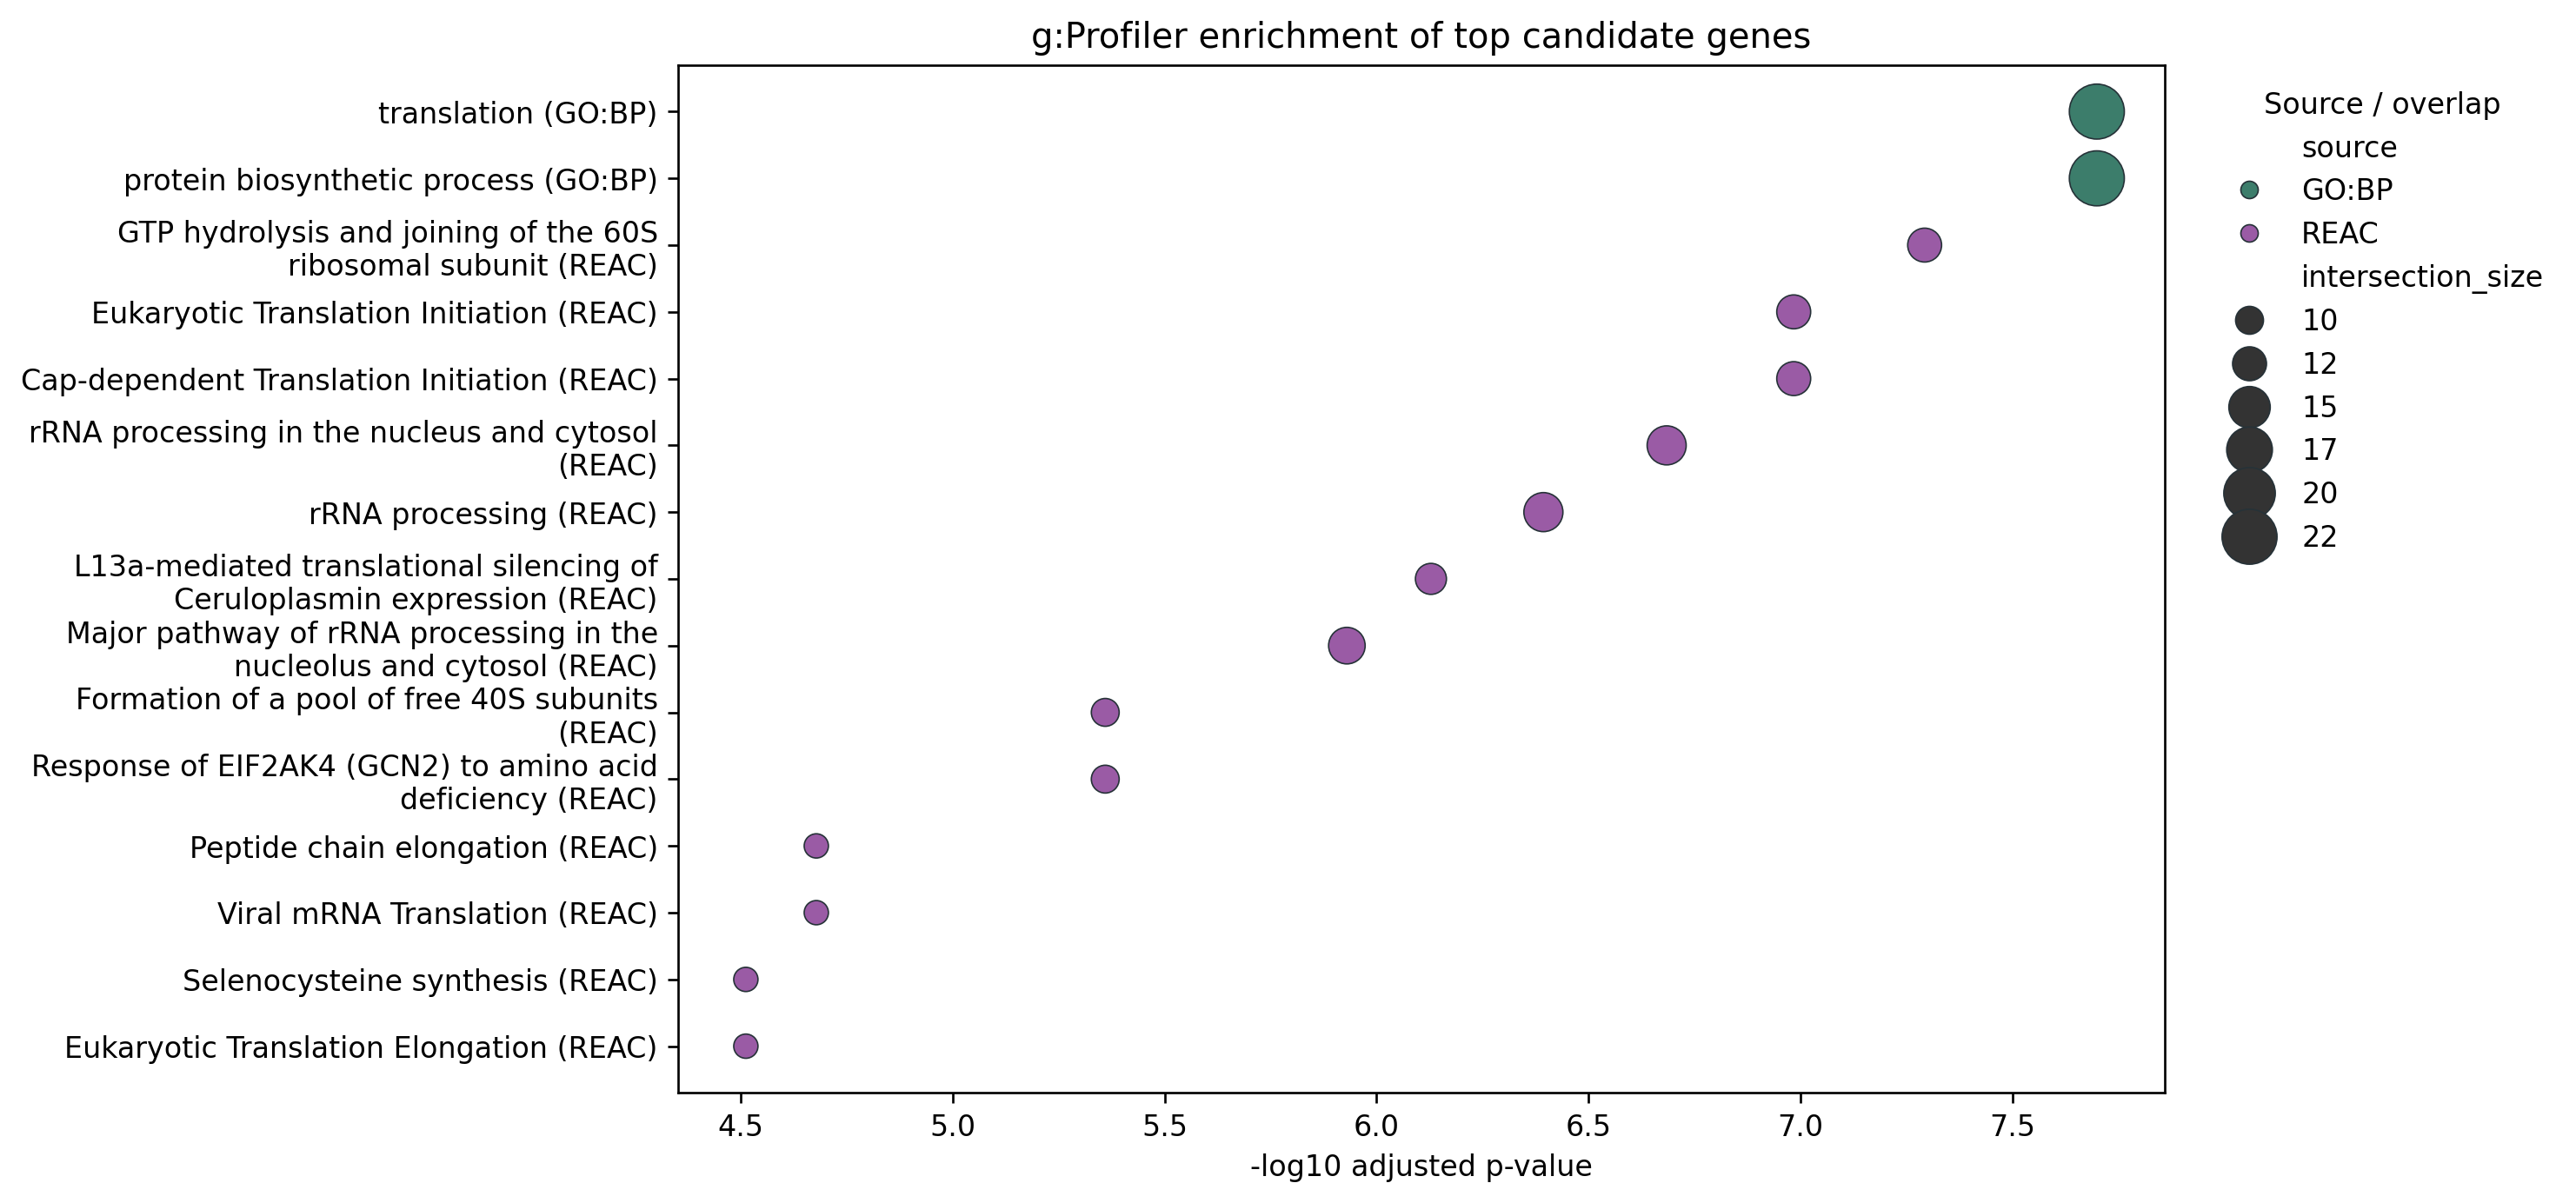
\includegraphics[width=0.88\linewidth]{../figures/candidate_enrichment_terms.png}
  \caption{g:Profiler GO biological process and Reactome enrichment among top
  candidate genes. Point size shows candidate-gene overlap with each term;
  the x-axis shows enrichment significance ($-\log_{10}$ adjusted $p$-value).}
  \label{fig:enrichment}
\end{figure}
